
\chapter*{ಹಿನ್ನುಡಿ}

\thispagestyle{plain}

ರಾಮನ್ ಅವರ ಜೀವನವು ಹಲವಾರು ವಿಧಗಳಲ್ಲಿ ಅಸಾಮಾನ್ಯವಾದುದು. ಆದರೆ ಈ ಅಸಾಮಾನ್ಯ ಜೀವನಾವಧಿಯಲ್ಲಿ ಅವರು ವಿಜ್ಞಾನದಲ್ಲಿ ತೊಡಗಿಸಿಕೊಂಡದ್ದೂ ಆಕಸ್ಮಿಕವೇ. ಹಿಂತಿರುಗಿ ನೋಡಿದಾಗ ಅವರು ವಿಜ್ಞಾನವನ್ನೇ ಏಕೆ ಆಯ್ದುಕೊಂಡರು ಎಂಬುದು ವೇದ್ಯವಾಗುತ್ತದೆ. ಅವರಿಗೆ ಭೌತ ವಿಜ್ಞಾನದೆಡೆಗೆ ಅತ್ಯಪೂರ್ವ ಸೆಳೆತವಿತ್ತು. ಅವರಲ್ಲಿನ ಸೃಜನ ಶೀಲ ಪಿಪಾಸೆಯು ಈ ವಿಜ್ಞಾನ ಶಿಸ್ತಿನಲ್ಲಿ ಅವಕಾಶಗಳನ್ನು ಶೋಧ ಮಾಡತೊಡಗಿತು. ಆದರೆ ಒಬ್ಬ ವ್ಯಕ್ತಿಯ ವಿಧಿ ಎನ್ನುವುದು ಅವನೊಳಗಿನ ಸ್ವತಂತ್ರ ಕರ್ತೃತ್ವಶಕ್ತಿ ಮತ್ತು ಅವನಿಗೊದಗಿಬರುವ ಅವಕಾಶಗಳು ಮತ್ತು ಸಂದರ್ಭಗಳ ಮೇಲೆ ಅವಲಂಬಿತವಾಗಿರುತ್ತದೆ. ಅವಕಾಶ/ಸಂದರ್ಭಗಳು ಒದಗಿ ಬರುವುದು ಯಾದೃಚ್ಛಿಕವಾಗಿ. ವ್ಯಕ್ತಿಗೆ ಇವುಗಳ ಮೇಲೆ ಯಾವುದೇ ಹಿಡಿತವಿರುವುದಿಲ್ಲ. ಯಾವುದೇ ವ್ಯಕ್ತಿಯ ಜೀವನದಲ್ಲಿ ಈ ಅಂಶಗಳೇ ಪ್ರಧಾನ ಪಾತ್ರವಹಿಸುತ್ತವೆ. ರಾಮನ್ ಅವರ ಜೀವನದಲ್ಲಿ ಹೀಗೆಯೇ ಆಗಿದೆ. ರಾಮನ್ ಅವರಿಗೆ ಸರ್ಕಾರದ ಹಣಕಾಸು ವಿಭಾಗದಲ್ಲಿ ಸಿಕ್ಕ ಕೆಲಸದಿಂದಾಗಿ, ಜೀವನೋಪಾಯಕ್ಕಾಗಿ ಪರದಾಡಬೇಕಾದ ಸಂದರ್ಭವೊದಗಲಿಲ್ಲ. ಈ ಹಣಕಾಸಿನ ಭದ್ರತೆ ಮತ್ತು ಕಲ್ಕತ್ತಾ ನಗರವಾಸವು ಅವರಿಗೆ ಇಷ್ಟವಾದ ಚಟುವಟಿಕೆಗಳಲ್ಲಿ ತೊಡಗಿಸಿಕೊಳ್ಳಲು ಅನುವುಮಾಡಿ ಕೊಟ್ಟಿತು.

ಅಂದಿನ ದಿನಗಳಲ್ಲಿ ಬೌದ್ಧಿಕ ಮತ್ತು ಸಾಂಸ್ಕೃತಿಕ ಪರಿಸರಕ್ಕಾಗಿ ಕಲ್ಕತ್ತ ನಗರವು ಹೆಸರು ಮಾಡಿತ್ತು. ವಿಜ್ಞಾನ ಚಟುವಟಿಕೆಗಳು ಬೌದ್ಧಿಕ ವಲಯಗಳಲ್ಲಿ ಗೌರವಾನ್ವಿತ ಹವ್ಯಾಸವೆನಿಸಿತ್ತು. ಇದರ ಬಗ್ಗೆ ರಾಮನ್‍ರವರು ಹೀಗೆಂದಿದ್ದರು “ಒಂದು ಪ್ರಸಿದ್ಧ ನಗರವು ಮತ್ತು ಅದರ ಜನತೆಯು ವೈಜ್ಞಾನಿಕ ಪರಿಸರಕ್ಕೆ ಅನುವುಮಾಡಿ ಕೊಡಬಲ್ಲುದೇ ಎಂಬುದು ಪ್ರಶ್ನಾರ್ಥಕ ವಿಷಯವಾಗಿದೆ. ಇದಕ್ಕೆ ಇಲ್ಲ ಎಂಬ ಉತ್ತರವೇ ಸಾಧುವೆನ್ನಿಸಬಹುದು. ಇದಕ್ಕೆ ಹಲವಾರು ನಿದರ್ಶನಗಳೂ ಇವೆ. ಬ್ರಿಟನ್ ನಲ್ಲಿಯೂ ಸಹ ವೈಜ್ಞಾನಿಕ ವಾತಾವರಣ ಇರುವುದು ಕೇಂಬ್ರಿಡ್ಜ್ ನಲ್ಲಿಯೇ ಹೊರತು ಲಂಡನ್ ಅಥವಾ ಎಡಿನ್ ಬರ್ಗ್ ನಂತಹ ಪ್ರಸಿದ್ಧ ನಗರಗಳಲ್ಲಲ್ಲ. ಇದು ಆಕಸ್ಮಿಕವೇನಲ್ಲ. ಆದರೆ ಪ್ಯಾರಿಸ್ ನಗರ ಹಾಗಿಲ್ಲ, ಅದು ನಿಜಕ್ಕೂ ದೇಶದ ರಾಜಕೀಯ, ಸಾಂಸ್ಕೃತಿಕ ಮತ್ತು ವೈಜ್ಞಾನಿಕ ರಾಜಧಾನಿ. ಬಂಗಾಳ ಪ್ರಾಂತ್ಯದ ಮಟ್ಟಿಗೆ ಕಲ್ಕತ್ತಾನಗರವು ಇದೇ ಬಗೆಯಲ್ಲಿದೆ. ಒಂದಾನೊಂದು ಕಾಲದಲ್ಲಿ ಈ ನಗರವು ಬ್ರಿಟಿಷ್ ಸಾಮ್ರಾಜ್ಯದ ರಾಜಧಾನಿಯಾಗಿದ್ದದ್ದು, ವೈಜ್ಞಾನಿಕ ರಂಗದ ಮಟ್ಟಿಗೆ ಹಾಗೆಯೇ ಮುಂದುವರಿಯುತ್ತಿರುವುದು ನೋಡುಗರಿಗೆ ಎದ್ದು ಕಾಣುತ್ತದೆ. ಕಲ್ಕತ್ತಾ ನಗರದ ಪ್ರತಿಷ್ಠೆ ಮತ್ತು ಪ್ರಭಾವವು ಶತಮಾನಗಳಿಂದ ಮುಂದುವರಿಸಿಕೊಂಡು ಬಂದ ಶಿಕ್ಷಣದ ಮತ್ತು ಜ್ಞಾನ ಪಿಪಾಸೆಯ ಸಂಪ್ರದಾಯಗಳಿಂದಲೂ ಮತ್ತು ಈ ನಗರವನ್ನು ಶ‍್ರೀಮಂತಗೊಳಿಸಿದ ಶಿಕ್ಷಣವೇತ್ತರೂ ಪಂಡಿತರೂ, ಬುದ್ಧಿಜೀವಿಗಳಿಂದ (ಭಾರತೀಯ\enginline{--}ಯೂರೋಪೀಯ) ಬೆಳೆದು ಬಂದಿದೆ. ಡಾ।। ಮಹೇಂದ್ರ ಲಾಲ ಸರ್ಕಾರ್, ಸರ್ ಆಶುತೋಷ ಮುಖರ್ಜಿ ಮತ್ತು ಇಂತಹ ನೂರಾರು ವಿದ್ವಾಂಸರು ಉನ್ನತ ಶಿಕ್ಷಣ ಮತ್ತು ಸಂಶೋಧನೆಗಳಿಗಾಗಿ ಹಾಕಿದ ಶ್ರಮದ ಫಲವನ್ನು ಇಂದು ಜನತೆಯು ಅನುಭವಿಸುವಂತಾಗಿದೆ.”

ಇಂತಹ ಬೌದ್ಧಿಕವಾದ ವಾತಾವರಣವಿಲ್ಲದೆ, ಇಂಡಿಯನ್ ಅಸೋಸಿಯೇಷನ್ ಫಾರ್\break ಕಲ್ಟಿವೇಷನ್ ಆಫ್ ಸಯನ್ಸ್ ಸಾಧ್ಯವಾಗುತ್ತಿರಲಿಲ್ಲ. ಈ ಸಂಸ್ಥೆಯ ಮೂಲಕವೇ ರಾಮನ್‍ರವರು ತಮ್ಮ ಭೌತಶಾಸ್ತ್ರದ ಆಸಕ್ತಿಯನ್ನು ಮುಂದುವರಿಸುವಂತಾಯಿತು. ಇಂತಹ ಸಂಸ್ಥೆಯೊಂದು ನಗರದಲ್ಲಿದ್ದು ಅದರ ಪರಿಚಯವು ರಾಮನ್‍ರವರಿಗೆ ಆದದ್ದೇ ಒಂದು ಆಕಸ್ಮಿಕ ಘಟನೆಯಾಗಿತ್ತು. ಈ ಸಂಸ್ಥೆಯು ತನ್ನ ತೆರೆದ ಬಾಹುಗಳಿಂದ ಸ್ವಾಗತಮಾಡಿದ್ದಷ್ಟೇ, ರಾಮನ್‍ರವರಿಗೆ ಬೇಕಾದ ಉತ್ತೇಜನವಾಗಿತ್ತು. ಇವೆರಡೂ ರಾಮನ್‍ರವರ ಜೀವನದಲ್ಲಿನ ಮಹತ್ವದ ತಿರುವುಗಳು. ರಾಮನ್‍ರವರ ವ್ಯಕ್ತಿತ್ವಕ್ಕೆ ಹೇಳಿಮಾಡಿಸಿದಂತೆ ಈ ಸಂಸ್ಥೆ ಇದ್ದಿತು. ರಾಮನ್‍ರವರು ಇಲ್ಲಿ ತಮ್ಮ ಕಾರ್ಯಕ್ಕೆ ಸಂಪೂರ್ಣ ಸ್ವಾತಂತ್ರ್ಯವನ್ನು ಅನುಭವಿಸಿದರು. ಅವರಿಗೆ ಸಿಕ್ಕ ಮುಕ್ತ ಅವಕಾಶದಿಂದಲೇ ಉನ್ನತ ಕ್ರಿಯಾಶೀಲತೆ ಸಿದ್ಧಿಸಿತು.

ರಾಮನ್‍ರವರಿಗೆ ವಿಜ್ಞಾನದಲ್ಲಿ ತೀವ್ರ ಒಲವು ಮತ್ತು ಅದಮ್ಯ ಆಸಕ್ತಿಯಿತ್ತು. ಮುಕ್ತ ಆಲೋಚನೆ, ಸಂಕಲ್ಪ ಶಕ್ತಿ, ದಣಿವರಿಯದ ದುಡಿತ ಮತ್ತು ಕತೃತ್ವಶಕ್ತಿಗಳು ವಿಜ್ಞಾನದ ಸಾಧನೆಗೆ ಆಧಾರ ಸ್ಥಂಬಗಳು. ವಿಜ್ಞಾನದಲ್ಲಿ ರಾಮನ್‍ರವರ ಒಳನೋಟಗಳು, ಅವರನ್ನು ಪ್ರಮುಖ ವೈಜ್ಞಾನಿಕ ಸಮಸ್ಯೆಗಳ ಸಂಶೋಧನೆಯತ್ತ ಸೆಳೆದವು. ತಮಗಿದ್ದ ಅಲ್ಪ ವೈಜ್ಞಾನಿಕ ಸಾಮಗ್ರಿಯನ್ನು ಬಳಸಿಕೊಂಡೇ ಈ ಸಂಶೋಧನೆಗಳಲ್ಲಿ ಸಿದ್ಧಿ ಪಡೆದರು. ಅವರು ತೊಡಗಿಸಿಕೊಂಡ ವೈಜ್ಞಾನಿಕ ಕ್ಷೇತ್ರಗಳಲ್ಲಿ ಅಲ್ಪ ಉಪಕರಣಗಳಲ್ಲಿ ಉನ್ನತಮಟ್ಟದ ಸಂಶೋಧನೆಗಳನ್ನು ಮಾಡಿದರು. \enginline{1907} ರಿಂದ \enginline{1917}ರವರೆಗೆ ಅಸಿಸ್ಟಂಟ್ ಅಕೌಂಟಂಟ್ ಜನರಲ್ ಆಗಿ ಬಿಡುವಿಲ್ಲದ ಸಶ್ರಮ ದುಡಿತವಿದ್ದರೂ ಸಹ ತಮ್ಮ ವೈಜ್ಞಾನಿಕ ಚಟುವಟಿಕೆಗಳಿಗೆ ಸಮಯ ಉಳಿಸಿಕೊಂಡರು. ತಮ್ಮ ಕಛೇರಿಯ ದುಡಿತದಿಂದ ಉಳಿದ ಸಮಯದಲ್ಲಿ, ಇಂಡಿಯನ್ ಅಸೋಸಿಯೇಷನ್ ಫಾರ್ ಕಲ್ಟಿವೇಷನ್ ಆಫ್ ಸಯನ್ಸ್ ನಲ್ಲಿ ವೈಜ್ಞಾನಿಕ ಅಧ್ಯಯನವನ್ನು ಮುಂದುವರೆಸಿದರು. ಅಲ್ಲಿ ಶ್ರಮವಹಿಸಿ ಪ್ರಯೋಗಶಾಲೆಯನ್ನು ಸಿದ್ಧಗೊಳಿಸಿದರು. ಅಲ್ಲಿ ಪ್ರಯೋಗಗಳನ್ನು ಮಾಡಿ, ಸಂಶೋಧನಾ ಪ್ರಬಂಧಗಳನ್ನು ಪ್ರಕಟಿಸಿದರು.

ತಾವು ಬೆಳಕು ಮತ್ತು ಧ್ವನಿಗಳ ವಿಷಯಗಳಲ್ಲಿ ಕೈಗೊಂಡ ಪ್ರಯೋಗಗಳು ಫಲನೀಡತೊಡಗಿದ ಮೇಲೆ ಅವರಿಗೆ ತಮ್ಮ ವೈಜ್ಞಾನಿಕ ಪ್ರಯೋಗಶೀಲತೆ ಮತ್ತು ಸಂಶೋಧನಾ ಸಾಮರ್ಥ್ಯಗಳ ಬಗ್ಗೆ ತೀವ್ರ ನಂಬಿಕೆ ಹುಟ್ಟಿತು. ಸ್ವಂತಿಕೆಯಿಂದ ಮುಂದುವರಿಯಬಲ್ಲೆನೆಂಬ ಧೈರ್ಯದಿಂದ ತಮ್ಮ ಉದ್ಯೋಗವನ್ನು ತೊರೆಯಲು ಮುಂದಾದರು. ಅವರನ್ನು ಪಾಲಿತ್ ಪ್ರೊಫೆ಼ಸರ್ ಎಂದು ನೇಮಿಸಿದಾಗ, ರಾಮನ್‍ರವರು ಪೂರ್ಣಾವಧಿಯ ವಿಜ್ಞಾನ ಸಂಶೋಧಕರಾಗಿ ಹೊರಹೊಮ್ಮಿದರು.

ಬೆಳಕಿನ ಚದರುವಿಕೆ ಮತ್ತು ದ್ಯುತಿ ವಿಜ್ಞಾನಗಳಲ್ಲಿ ತೀವ್ರ ಸಂಶೋಧನಾ ಸಾಧ್ಯತೆಗಳಿವೆಯೆಂದು ಮನಗಂಡು, ತಮ್ಮ ಕ್ಷೇತ್ರವನ್ನು ಧ್ವನಿ ಸಂಶೋಧನಾ ರಂಗದಿಂದ ಬದಲಿಸಿಕೊಂಡರು. ಇದರ ಬಗ್ಗೆ \enginline{1968}ರಲ್ಲಿ ಹೀಗೆ ನೆನಪಿಸಿಕೊಂಡರು.

\newpage

“ನನ್ನ ವಿಜ್ಞಾನ ವ್ಯವಸಾಯದಲ್ಲಿ ತಂತಿ ವಾದ್ಯಗಳಲ್ಲಿನ ಸಂಶೋಧನೆಯನ್ನು ಆರಂಭಿಕ ಹಂತ\break ವೆಂದು ತಿಳಿದಿದ್ದೇನೆ. ಇವು \enginline{1914} ರಿಂದ \enginline{1918} ರವರೆಗೆ ನಡೆಸಿದ ಚಟುವಟಿಕೆಗಳು. ಜುಲೈ \enginline{1917}ರಲ್ಲಿ ನನಗೆ ಫ್ರೊಫೆಸರ್ ಆಗಲು ಆಹ್ವಾನ ಬಂದ ಬಳಿಕ ಮತ್ತು ದ್ಯುತಿ ವಿಜ್ಞಾನದ ಕಡೆಗೆ ನನ್ನ ಆಸಕ್ತಿಯು ಹೊರಳಿತು. ಪಿಟೀಲು ಮಾದರಿಯ ತಂತಿ ವಾದ್ಯಗಳ ಸಂಶೋಧನೆಯು ನನ್ನಿಂದ ಹಿಂದೆ ಸರಿಯಿತು”.

ಅವರಿಗೆ ವಿಜ್ಞಾನದ ಅಂತರ್ಗತ ಸೌಂದರ್ಯದ ಬಗ್ಗೆ ಸೆಳೆತವಿತ್ತು. ಹಿಂದಿನ ವಿಜ್ಞಾನಿಗಳ ಪೈಕಿ ಲಾರ್ಡ್ ರ‍್ಯಾಲೈ ಅವರಿಗೆ ಮಾದರಿಯಾಗಿದ್ದರು. ಇದರಿಂದಾಗಿ ಬೆಳಕಿನ ಚದರಿಕೆಯ ಬಗ್ಗೆ ಅವರ ಸಂಶೋಧನೆ ಮೊದಲಾಯಿತು. ಅವರ ಜೊತೆಗಾರರೊಂದಿಗೆ ಎಂಟು ವರ್ಷಗಳ ಕಾಲ ಈ ನಿಟ್ಟಿನಲ್ಲಿ ಪ್ರಯೋಗಗಳನ್ನು ಮುಂದುವರಿಸಿದರು. ತಾಳ್ಮೆ, ಗುಣಾತ್ಮಕ ವಿಶ್ಲೇಷಣೆ ಮತ್ತು ನವೀನ ಸಂಶೋಧನಾ ಮಾರ್ಗಗಳನ್ನು ಹಂತಹಂತವಾಗಿ ಶೋಧಿಸಿಕೊಳ್ಳುತ್ತಾ ಮುಂದುವರೆದಂತೆ, ಈ ರಂಗದಲ್ಲಿ ಅತಿ ವಿಶಿಷ್ಟ ಮತ್ತು ಅವರಿಗೆ ಪ್ರಖ್ಯಾತಿ ನೀಡಿದ ಸಂಶೋಧನೆಯನ್ನು ಮಾಡಲು ಸಾಧ್ಯವಾಯಿತು. ಗಮನಿಸಬೇಕಾದ ಅಂಶವೆಂದರೆ ರಾಮನ್‍ರವರು ಅತ್ಯುನ್ನತ ಮಟ್ಟದ ಪ್ರಯೋಗಶೀಲ ವಿಜ್ಞಾನಿ. ಇದು ಅವರ ಸಾಧನೆಯೇ ಸರಿ. ಏಕೆಂದರೆ ಕಾಲೇಜಿನ ದಿನಗಳಲ್ಲೂ ಸಹ ಅವರಿಗೆ ಪ್ರಯೋಗ ರಂಗದಲ್ಲಿ ಯಾವುದೇ ತರಬೇತಿ ಸಿಕ್ಕಿರಲಿಲ್ಲ. ಇಂದೂ ಸಹ ಯಾವುದೇ ಭಾರತೀಯ ವಿಶ್ವವಿದ್ಯಾನಿಲಯಗಳಲ್ಲಿ\break  ಪ್ರಯೋಗಶೀಲತೆ ಕಂಡುಬರುವುದಿಲ್ಲ. ಬರೀ ಪುಸ್ತಕದ ಓದಿಗಷ್ಟೇ ಸೀಮಿತವಾದ ಶಿಕ್ಷಣ\break ನೀಡಲಾಗುತ್ತದೆ.

ವೈಜ್ಞಾನಿಕ ಮನೋಧರ್ಮವು ಮುಖ್ಯವಾಗಿ ಪ್ರಕೃತಿಯ ಬಗೆಗಿನ ಕುತೂಹಲದಿಂದ ಮೊದಲ ಹೆಜ್ಜೆಯಿಡುತ್ತದೆ. ನೈಸರ್ಗಿಕ ಪ್ರಕ್ರಿಯೆಗಳ ಬಗೆಗಿನ ತೀವ್ರ ಆಸಕ್ತಿಯು ಹರಳುಗಟ್ಟುತ್ತದೆ. ಪ್ರಯೋಗ\-ಶೀಲತೆ, ವೀಕ್ಷಣೆ ಮತ್ತು ವಿಶ್ಲೇಷಣೆಗಳು ವೈಜ್ಞಾನಿಕ ಪದ್ಧತಿಯ ಸೋಪಾನಗಳಾಗಿವೆ. ತಾಳ್ಮೆ ಮತ್ತು ಸಂಲಗ್ನತೆಗಳು ಮಾರ್ಗದಲ್ಲಿ ಮುನ್ನಡೆಸುವ ಊರುಗೋಲುಗಳಾಗಿವೆ. ತಮ್ಮ ಜೀವನ ಮತ್ತು ಕಾರ್ಯಶೀಲತೆಗಳಲ್ಲಿ ರಾಮನ್‍ರವರು ಒಬ್ಬ ನೈಜ ವಿಜ್ಞಾನಿಯ ಆಲೋಚನೆಗಳು, ಕಾರ್ಯವೈಖರಿ ಮತ್ತು ನಡತೆಯನ್ನು ತೋರಿಸಿಕೊಟ್ಟರು. ಒಂದು ಕ್ಷಣವೂ ಸಹ ವಿಜ್ಞಾನದಲ್ಲಿ ತಮ್ಮ ಆಸಕ್ತಿಯನ್ನು ಕಳೆದುಕೊಳ್ಳಲಿಲ್ಲ. ಆದರೆ ತಮ್ಮ ಜೀವನದುದ್ದಕ್ಕೂ ಎದುರಾದ, ಸೋಲು ಮತ್ತು ಹತಾಶೆಗಳಿಗೆ ಕುಗ್ಗಲಿಲ್ಲ.

ರಾಮನ್‍ರವರು ಹೇಳಿಕೊಳ್ಳುವಂತಹ ವಿನಯಶೀಲರಾಗಿರಲಿಲ್ಲ. ಬದಲಿಗೆ ಅವರು ಬಹಳ ಗರ್ವಿಷ್ಠರು. ಹೊಗಳಿಕೆಗೆ ತಲೆತೂಗುವವರು. ಕೆಲವೊಮ್ಮೆ ಅಸಾಧ್ಯ ಕೋಪ ಪ್ರದರ್ಶಿಸುತ್ತಿದ್ದರು. ಆಗ ನಾಲಗೆಯ ಮೇಲೆ ಹಿಡಿತವಿರುತ್ತಿರಲಿಲ್ಲ. ಈ ಬಗೆಯ ಗುಣಗಳಿಗೆ ತೀವ್ರ ಪ್ರತಿಕ್ರಿಯೆ ಎದುರಿಸಬೇಕಾಗುತ್ತಿತ್ತು. ಆದರೆ ಅವರ ಹತ್ತಿರದವರಿಗೆ, ಅವರಲ್ಲಿನ ವಿಜ್ಞಾನಿಯೊಬ್ಬನ ಗುಣಗಳೂ ಮತ್ತು ಪ್ರಕೃತಿಯನ್ನು ಆರಾಧಿಸುವ ಪರಿಯೂ ಈ ಕೊರತೆಗಳನ್ನು ಮೀರಿ ಆಲೋಚಿಸುವಂತೆ ಮಾಡುತ್ತಿತ್ತು.

ಅವರ ಜೀವನೋತ್ಸಾಹ, ಸರಳತೆ ಮತ್ತು ನೇರ ನುಡಿಗಳು ಅವರ ಹತ್ತಿರ ಬಂದ ಎಲ್ಲರನ್ನೂ ಸೆಳೆಯುತ್ತಿತ್ತು.

\newpage

\heading{ಸಿ. ವಿ. ರಾಮನ್‍ರವರ ಜೀವನದಲ್ಲಿ ಕೆಲವು ಮುಖ್ಯ ದಿನಗಳು}

\begin{longtable}{@{}lcp{6.7cm}<{\raggedright}@{}}
\general{\enginline{1888}} ನವೆಂಬರ್ \general{\enginline{2}}  &  \general{\enginline{—}}  &  ತಿರುವಣೈಕ್ಕಾವಲ್, ತಿರುಚಿನಾಪಳ್ಳಿಯ ಹತ್ತಿರ ಜನನ \\
\general{\enginline{1892–1902}}  &  \general{\enginline{—}}  &  ವಿಶಾಖಪಟ್ಟಣದಲ್ಲಿ ಮೊದಲ ಶಿಕ್ಷಣ \\
\general{\enginline{1900}}  &  \general{\enginline{—}}  &  ಮೆಟ್ರಿಕ್ ಪರೀಕ್ಷೆ \\
\general{\enginline{1902}}  &  \general{\enginline{—}}  &  ಎಫ್.ಎ. ಪರೀಕ್ಷೆ, ಪ್ರೆಸಿಡೆನ್ಸಿ ಕಾಲೇಜು ಮದರಾಸ್‍ಗೆ ಸೇರ್ಪಡೆ \\
\general{\enginline{1904}}  &  \general{\enginline{—}}  &  ಬಿ.ಎ. ಮೊದಲ ಚಿನ್ನದ ಪದಕ \\
\general{\enginline{1906}}  &  \general{\enginline{—}}  &  ಫಿಲಾಸೊಫಿಕಲ್ ಮ್ಯಾಗಜಿನ್, ಲಂಡನ್‍ನಲ್ಲಿ ಮೊದಲ ಸಂಶೋಧನ ಲೇಖನ ಪ್ರಕಟ \\
\general{\enginline{1907}}  &  \general{\enginline{—}}  &  ಎಂ.ಎ. ಮೊದಲ ರ‍್ಯಾಂಕ್, ಫೈನಾನ್ಸಿಯಲ್ ಸಿವಿಲ್ ಸರ್ವೀಸ್ ಪರೀಕ್ಷೆ \\
 &  \general{\enginline{—}}  &  ಲೋಕ ಸುಂದರಿಯೊಂದಿಗೆ ಮದುವೆ  \\
 &  \general{\enginline{—}}  &  ಕಲ್ಕತ್ತದ, ಫೈನಾನ್ಸ್ ಡಿಪಾರ್ಟ್‌ಮೆಂಟ್‍ನಲ್ಲಿ, ಅಸಿಸ್ಟೆಂಟ್ ಅಕೌಂಟೆಂಟ್ ಜನರಲ್ ಆಗಿ ನೇಮಕ \\
 &  \general{\enginline{—}}  &  ಇಂಡಿಯನ್ ಅಸೋಸೊಯೇಶನ್ ಫಾರ್ ಕಲ್ಟಿವೇಶನ್ ಆಫ್ ಸೈನ್ಸ್ ನಲ್ಲಿ ಕೆಲಸ ಶುರು \\
\general{\enginline{1907–1917}}  &  \general{\enginline{—}}  &  ಅಧಿಕಾರಿ, ಫೈನಾನ್ಸ್ ಡಿಪಾರ್ಟ್‌ಮೆಂಟ್ ಕಲ್ಕತ್ತ, ರಂಗೂನ್, ನಾಗಪುರ ಮತ್ತೆ ಕಲ್ಕತ್ತ \\
\general{\enginline{1917}} ಜುಲೈ  &  \general{\enginline{—}}  &  ಪಲಿತ್ ಫ್ರೊಫೆಸರ್, ಕಲ್ಕತ್ತ ಯೂನಿವರ್ಸಿಟಿ \\
\general{\enginline{1919}}  &  \general{\enginline{—}}  &  ಸೆಕ್ರೆಟರಿ \general{\enginline{IACS}} \\
\general{\enginline{1921}}  &  \general{\enginline{—}}  &  ವಿದೇಶಕ್ಕೆ ಮೊದಲ ಪಯಣ ಇಂಗ್ಲೆಂಡ್‍ಗೆ \\
\general{\enginline{1924}}  &  \general{\enginline{—}}  &  ಲಂಡನ್ ನ ರಾಯಲ್ ಸೊಸೈಟಿಗೆ ಚುನಾಯಿತರಾದದ್ದು \\
\general{\enginline{1928}} ಫೆಬ್ರವರಿ \general{\enginline{28}}  &  \general{\enginline{—}}  &  ಕಲ್ಕತ್ತದಲ್ಲಿ ರಾಮನ್ ಪರಿಣಾಮದ ಆವಿಷ್ಕಾರ \\
\general{\enginline{1928}} ಮಾರ್ಚ್ \general{\enginline{16}}  &  \general{\enginline{—}}  &  ಬೆಂಗಳೂರಿನ ಸೆಂಟ್ರಲ್ ಕಾಲೇಜಿನಲ್ಲಿ ಸೌತ್ ಇಂಡಿಯನ್ ಸೈನ್ಸ್ ಅಸೋಸಿಯೇಶನ್ ನಲ್ಲಿ ರಾಮನ್ ಪರಿಣಾಮದ ಬಗ್ಗೆ ಮೊದಲ ಸಾರ್ವಜನಿಕ ಉಪನ್ಯಾಸ \\
\general{\enginline{1929}}  &  \general{\enginline{—}}  &  ಬ್ರಿಟಿಷ್ ಸರ್ಕಾರದಿಂದ ನೈಟ್ ಹುಡ್ \\
\general{\enginline{1930}}  &  \general{\enginline{—}}  &  ಭೌತಶಾಸ್ತ್ರದಲ್ಲಿನ ನೊಬೆಲ್ ಬಹುಮಾನ \\
 &  \general{\enginline{—}}  &  ರಾಯಲ್ ಸೊಸೈಟಿಯ ಹ್ಯೂಸ್ ಪ್ರೈಸ್ \\
\general{\enginline{1933}} ಮಾರ್ಚ್ \general{\enginline{31}}  &  \general{\enginline{—}}  &  ನಿರ್ದೇಶಕ, ಟಾಟಾ ವಿಜ್ಞಾನ ಸಂಸ್ಥೆ, ಬೆಂಗಳೂರು \\
\general{\enginline{1934}}  &  \general{\enginline{—}}  &  ರಾಮನ್‍ರವರರಿಂದ ಇಂಡಿಯನ್ ಅಕಾಡೆಮಿ ಆಫ್ ಸೈನ್ಸ್‌ನ ಸ್ಥಾಪನೆ \\
\general{\enginline{1935–36}}  &  \general{\enginline{—}}  &  ರಾಮನ್\general{\enginline{--}} ನಾಥ್ ಸಿದ್ಧಾಂತ \general{\enginline{--}}ಶಬ್ದಾತೀತ ತರಂಗಗಳ ವಿಸರಣ \\
\general{\enginline{1937}}  &  \general{\enginline{—}}  &  ಟಾಟಾ ವಿಜ್ಞಾನ ಸಂಸ್ಥೆಯ ನಿರ್ದೇಶಕ ಆಗಿ ಪದತ್ಯಾಗ, ಆದರೆ ಭೌತಶಾಸ್ತ್ರದ ಪ್ರೊಫೆ಼ಸರ್ ಮತ್ತು ಇಲಾಖೆಯ ಮುಖ್ಯಸ್ಥರಾಗಿ ಮುಂದುವರಿದರು \\
\general{\enginline{1940}}  &  \general{\enginline{—}}  &  ಕ್ವಾರ್ಟ್ಸ್ ಸ್ಪಟಿಕದಲ್ಲಿ ಸಾಫ್ಟ್ ಮೋಡನ್ನು ರಾಮನ್\general{\enginline{--}}ನೆಡುಂಗಾಡಿ ಜೋಡಿಯು ಆವಿಷ್ಕರಿಸಿದರು. \\
\general{\enginline{1942}}  &  \general{\enginline{—}}  &  ಫ್ರಾಂಕ್ಲಿನ್ ಮೆಡಲ್ \\
\general{\enginline{1948}} ಜುಲೈ  &  \general{\enginline{—}}  &  ಟಾಟಾ ವಿಜ್ಞಾನ ಸಂಸ್ಥೆಯಿಂದ ನಿವೃತ್ತಿ \\
 &  \general{\enginline{—}}  &  ರಾಮನ್ ರಿಸರ್ಚ್ ಇನ್ಸ್ಟಿಟ್ಯೂಟ್ ನ ಸ್ಥಾಪನೆ \\
 &  \general{\enginline{—}}  &  ನ್ಯಾಶನಲ್ ರಿಸರ್ಚ್ ಪ್ರೊಫೆ಼ಸರ್ ಹುದ್ದೆ \\
\general{\enginline{1954}}  &  \general{\enginline{—}}  &  ಭಾರತ ರತ್ನ \\
\general{\enginline{1957}}  &  \general{\enginline{—}}  &  ಅಂತಾರಾಷ್ಟ್ರೀಯ ಲೆನಿನ್ ಶಾಂತಿ ಪುರಸ್ಕಾರ, ಸೋವಿಯತ್ ಯೂನಿಯನ್ ನಿಂದ \\
\general{\enginline{1961}}  &  \general{\enginline{—}}  &  ವ್ಯಾಟಿಕನ್‍ನ ಪಾಂಟಿಫಿಕಲ್ ಅಕಾಡೆಮಿ ಆಫ್ ಸೈನ್ಸಸ್‍ಗೆ ಸದಸ್ಯರಾಗಿ ನೇಮಕ \\
\general{\enginline{1970}} ನವೆಂಬರ್ \general{\enginline{21}}  &  \general{\enginline{—}}  &  ಬೆಂಗಳೂರಿನಲ್ಲಿ ಮರಣ \\
\end{longtable}

\newpage

\heading{ಪದ ವಿವರಣಾ ಪಟ್ಟಿ}

\begin{longtable}{@{}lcp{6.7cm}<{\raggedright}@{}}
\general{\enginline{A.U.}}  &  \general{\enginline{–}}  &  ಆಂಗ್‍ಸ್ಟ್ರಾಮ್ ಯೂನಿಟ್ \general{\enginline{-}} \general{\enginline{\general{$10^\general{{-10}}$}}} ಮೀಟರ್ ತರಂಗಾಂತರದ ಅಳತೆ ಬೆಳಕಿನ ತರಂಗ ದೂರವನ್ನು ಅಳೆಯುವಾಗ ಬಳಸುವ ಅಳತೆ \\
\general{\enginline{Aromatic Compound}}  &  \general{\enginline{–}}  &  ಅಣುಗಳಲ್ಲಿ ಬೆನ್‍ಜೀನ್ ಉಂಗುರವಿರುವ ಸಂಯುಕ್ತ \\
\general{\enginline{Aliphatic Compound}}  &  \general{\enginline{–}}  &  ಉಂಗುರ ರಚನೆಯಿರುವ ಸಂಯುಕ್ತ \\
\general{\enginline{Anitrophy}}  &  \general{\enginline{–}}  &  ಸ್ಫಟಿಕಗಳಲ್ಲಿ ದಿಶೆಯನ್ನು ಅವಲಂಬಿಸಿ ವಿಭಿನ್ನ ಲಕ್ಷಣಗಳನ್ನು ಪ್ರಕಟಿಸುವ ಗುಣ \\
\general{\enginline{Alderman}}  &  \general{\enginline{–}}  &  ಬ್ರಿಟಿಷರ ಕಾಲದಲ್ಲಿ ನಗರ ಕಾರ್ಪೋರೇಷನ್ನಿನ ಉಪ ಮೇಯರ್ ಪಟ್ಟ \\
\general{\enginline{Amplitude}}  &  \general{\enginline{–}}  &  ಪಾರ \\
\general{\enginline{Amorphous}}  &  \general{\enginline{–}}  &  ಅಸ್ಫಟಿಕ \\
\general{\enginline{Blackhole of Culcutta}}  &  \general{\enginline{–}}  &  \general{\enginline{20}} ಜೂನ್ \general{\enginline{1756}}ರಲ್ಲಿ ಸಿರಾಜುದ್ದೌಲನು ಬಂಗಾಳದ ನವಾಬನಾಗಿದ್ದಾಗ, ಬ್ರಿಟಿಷ್ ಸೈನಿಕರನ್ನು ಫೋರ್ಟ್ ವಿಲಿಯಂನಲ್ಲಿ ಕೂಡಿ ಹಾಕಿದ್ದನು. ಇಲ್ಲಿ ಉಸಿರುಕಟ್ಟಿ \general{\enginline{123}} ಜನ ಸತ್ತಿದ್ದರು. \\
\general{\enginline{Brillouin Theory}}  &  \general{\enginline{–}}  &  ಬೆಳಕಿನ ಕಿರಣಗಳು ಹಾಯುವ ಮಾಧ್ಯಮದ ಅಣು/ಪರಮಾಣುಗಳು ಜಾಲಕದಿಂದ ರೂಪಾಂತರಗೊಳ್ಳುವುದು ಮತ್ತು ಚದರಿಕೆಗೆ ಒಳಗಾಗುವುದು \\
\general{\enginline{Brewsterian Angle}}  &  \general{\enginline{–}}  &  ಪಾರಕತಲದಿಂದ ಪ್ರತಿಫಲಿತವಾಗುವ ಬೆಳಕಿನ ಧ್ರುವೀಕರಣದ ಪ್ರಮಾಣವು, ಪ್ರತಿಫಲಿತ ಕಿರಣವು ವಕ್ರೀಭವನ ಕಿರಣಕ್ಕೆ ಲಂಬವಾಗಿರುವಾಗ ಗರಿಷ್ಠವಾಗಿರುತ್ತದೆ. ಈ ಗರಿಷ್ಠ ಧ್ರುವೀಕರಣ ಸಂಭವಿಸುವ ಆಪಾತ ಕೋನ. \\
\general{\enginline{Coherant}}  &  \general{\enginline{–}}  &  ಸಂಸಕ್ತ \\
\general{\enginline{Congenial}}  &  \general{\enginline{–}}  &  ಸಜಾತೀಯ \\
\general{\enginline{Compton effect}}  &  \general{\enginline{–}}  &  ಎಕ್ಸ್\general{\enginline{-}}ರೇ/ಗಾಮಾ ಕಿರಣಗಳ ಫೋಟಾನ್ಗಳು ಎಲೆಕ್ಟ್ರಾನ್ ಗಳಿಂದ ಚದರಿಸಲ್ಪಟ್ಟಾಗ ಫೋಟಾನ್‍ಗಳ ಶಕ್ತಿ ಕುಗ್ಗಿ ಎಲೆಕ್ಟ್ರಾನ್‍ಗಳ ಶಕ್ತಿ ಹಿಗ್ಗುವ ಪರಿಣಾಮ \\
\general{\enginline{Corpuscular theory}}  &  \general{\enginline{–}}  &  ಬೆಳಕಿನ ಕಣ ಸಿದ್ದಾಂತ \\
\general{\enginline{Crystal}}  &  \general{\enginline{–}}  &  ಸ್ಫಟಿಕ \\
\general{\enginline{Cleavage}}  &  \general{\enginline{–}}  &  ಭಾಗವಾಗು \\
\general{\enginline{Complementary}}  &  \general{\enginline{–}}  &  ಪೂರಕ \\
\general{\enginline{Dispersion}}  &  \general{\enginline{–}}  &  ಪ್ರಸರಣ \\
\general{\enginline{Diffusion}}  &  \general{\enginline{–}}  &  ವಿಸರಣ \general{\enginline{--}} ಅಣು/ಪರಮಾಣುಗಳು ಮಿಶ್ರಗೊಳ್ಳುವ ಪ್ರಕ್ರಿಯೆ. ಮಿಶ್ರಣವು ಸಮನಾಗಿ ಹಂಚಿಕೆಯಾಗುವುದು \\
\general{\enginline{Double Image Prism}}  &  \general{\enginline{–}}  &  ಐಸ್ ಲಾಂಡ್ ಸ್ಪಾರ್ ನಿಂದ ತಯಾರಿಸಿದ ಪಟ್ಟಕ ಪರಸ್ಪರ ಧ್ರುವೀಕರಣಗೊಂಡ ಎರಡು ಬಿಂಬಗಳನ್ನು ಹೊರಗೆಡಹುವುದು \\
\general{\enginline{Diffraction}}  &  \general{\enginline{–}}  &  ವಸ್ತುವಿನ ಅಂಚುಗಳನ್ನು ಬಳಸಿಕೊಂಡು ಬೆಳಕಿನ ತರಂಗಗಳು ಚಲಿಸುವ ಪ್ರಕ್ರಿಯೆ. ಬೆಳಕು ವಸ್ತುವಿನ ಅಂಚಿನ ಗುಂಟ ಬಾಗಿ ಚಲಿಸುವ ಕ್ರಿಯೆ \\
\general{\enginline{Florascence}}  &  \general{\enginline{–}}  &  ಪ್ರತಿದೀಪ್ತಿ \\
\general{\enginline{Filter}}  &  \general{\enginline{–}}  &  ಸೋಸುಕ \\
\general{\enginline{Heliostat}}  &  \general{\enginline{–}}  &  ಸೂರ್ಯ ಸ್ಥಿರ ದರ್ಶಕ \\
\general{\enginline{Hypothesis}}  &  \general{\enginline{–}}  &  ಆಧಾರ ಕಲ್ಪನೆ \\
\general{\enginline{Heterogeniety}}  &  \general{\enginline{–}}  &  ವಿಭಿನ್ನ \\
\general{\enginline{Incoherant}}  &  \general{\enginline{–}}  &  ಅಸಂಸಕ್ತ \\
\general{\enginline{Lamelle}}  &  \general{\enginline{–}}  &  ಪದರ \\
\general{\enginline{Lattice}}  &  \general{\enginline{–}}  &  ಜಾಲಕ \general{\enginline{--}} ಸ್ಫಟಿಕಗಳಲ್ಲಿ ಅಣುಗಳ/ಪರಮಾಣುಗಳ ಕ್ರಮಬದ್ಧ ಆವರ್ತನೀಯ ಜೋಡಣೆ \\
\general{\enginline{Lattice Dynamics}}  &  \general{\enginline{–}}  &  ಜಾಲಕ ಗತಿಶಾಸ್ತ್ರ \\
\general{\enginline{Mode}}  &  \general{\enginline{–}}  &  ಸಂಖ್ಯಾಗಣದಲ್ಲಿ ಹೆಚ್ಚುಸಲ ಪ್ರಕಟವಾಗುವ ಸಂಖ್ಯೆ ಬಹುವರ್ತಿ \\
\general{\enginline{Moonstone}}  &  \general{\enginline{–}}  &  ಚಂದ್ರಕಾಂತ ಶಿಲೆ \\
\general{\enginline{Nicole Prism}}  &  \general{\enginline{–}}  &  ಐಸ್ ಲಾಂಡ್ ಸ್ಟಾರ್ ಸ್ಪಟಿಕದಿಂದ ತಯಾರಿಸಿದ ಪಟ್ಟಕ. ಸ್ಪಟಿಕದ ಎರಡು ತುಂಡುಗಳನ್ನು ಜೋಡಿಸಿರುವುದರಿಂದ ಆಪಾತ ಬೆಳಕು ಎರಡು ಕಿರಣಗಳನ್ನು ನೀಡುತ್ತದೆ \\
\general{\enginline{Oscillation}}  &  \general{\enginline{–}}  &  ಆಂದೋಲನ \\
\general{\enginline{Opalascent}}  &  \general{\enginline{–}}  &  ಅಪಾರದರ್ಶಕ \\
\general{\enginline{Prism}}  &  \general{\enginline{–}}  &  ಪಟ್ಟಕ \\
\general{\enginline{Polarisation}}  &  \general{\enginline{–}}  &  ಧ್ರುವೀಕರಣ \\
\general{\enginline{Physiology}}  &  \general{\enginline{–}}  &  ಶರೀರ ವಿಜ್ಞಾನ \\
\general{\enginline{Rasette Technique}}  &  \general{\enginline{–}}  &  ಪಾದರಸದ ಬೆಳಕಿನ ಕಿರಣವನ್ನು ಬಳಸಿ ದ್ವಿತೀಯಕ ರೋಹಿತವನ್ನು ಪಡೆಯುವ ವಿಧಾನ \\
\general{\enginline{Spectrum}}  &  \general{\enginline{–}}  &  ರೋಹಿತ \\
\general{\enginline{Spectroscope}}  &  \general{\enginline{–}}  &  ರೋಹಿತದರ್ಶಕ \\
\general{\enginline{Sunstone}}  &  \general{\enginline{–}}  &  ಸೂರ್ಯಕಾಂತಿ ಶಿಲೆ \\
\general{\enginline{Sensitive}}  &  \general{\enginline{–}}  &  ಸಂವೇದಿ \\
\general{\enginline{Scattering}}  &  \general{\enginline{–}}  &  ಚದರುವಿಕೆ \\
\general{\enginline{Tyndall effect}}  &  \general{\enginline{–}}  &  ಬೆಳಕಿನ ಪಥದಲ್ಲಿ ಸೂಕ್ಷ್ಮ ಕಣಗಳು ಉಂಟು ಮಾಡುವ ಚದರಿಕೆ \\
\general{\enginline{Twinning}}  &  \general{\enginline{–}}  &  ಹೆಣಿಗೆ \\
\general{\enginline{Thermodynamics}}  &  \general{\enginline{–}}  &  ಉಷ್ಣಗತಿಶಾಸ್ತ್ರ \\
\end{longtable}

\newpage 
~ 

\thispagestyle{empty}


\misccmd

\begin{figure}[!htpb]
\centering
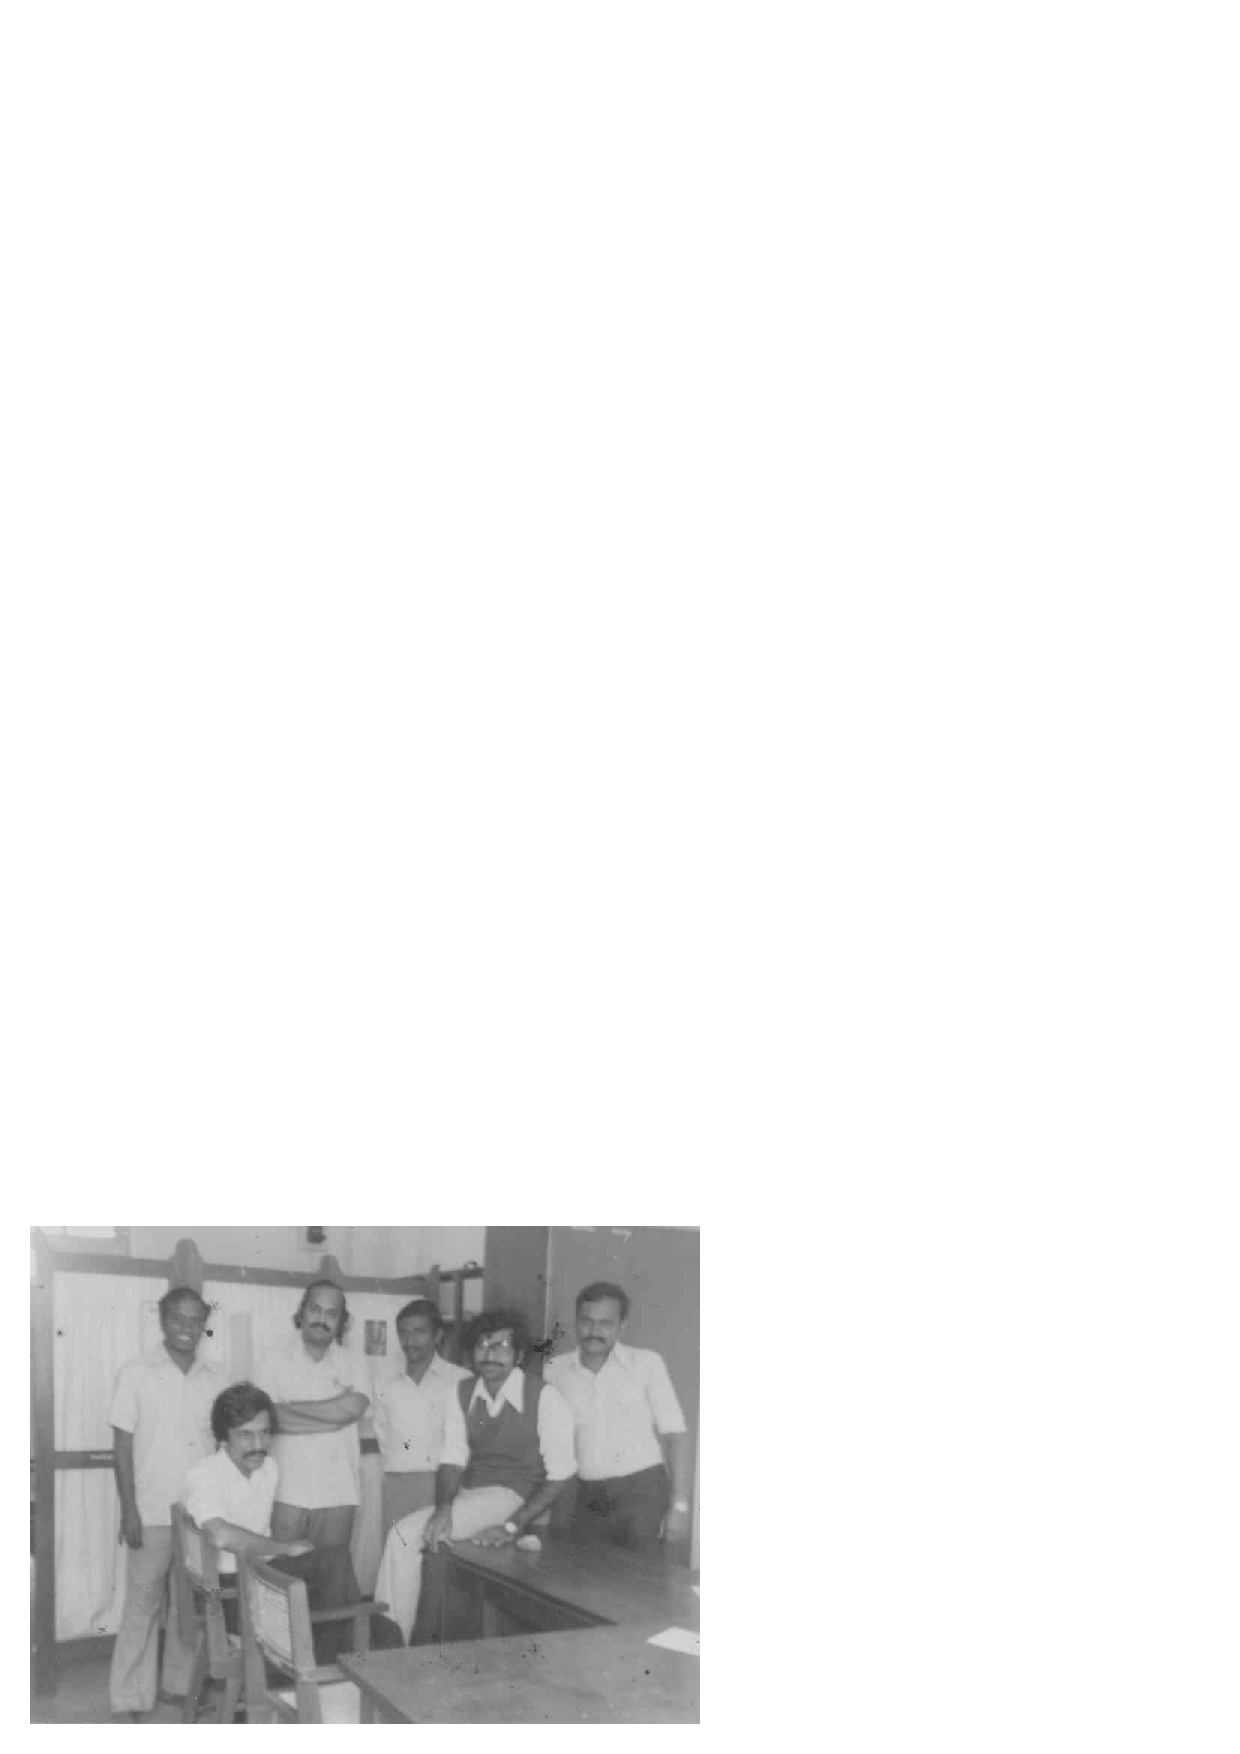
\includegraphics[scale=2.15]{"images/002.jpg"}
\end{figure}

\vfill

\misccmd

\begin{figure}[!htpb]
\centering
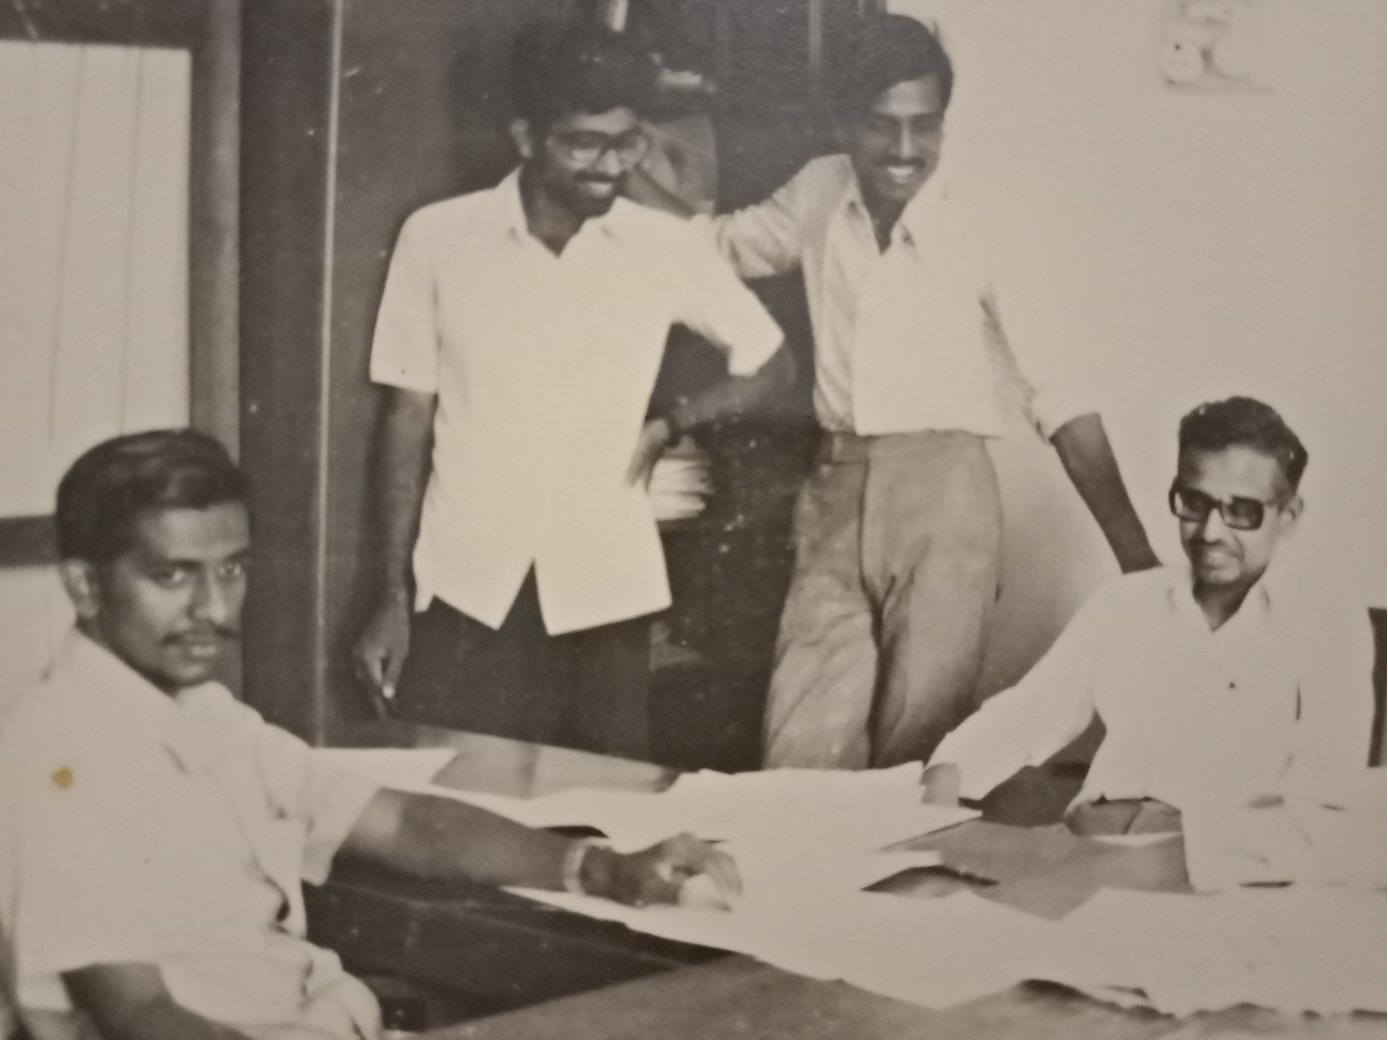
\includegraphics[scale=2.15]{"images/001.jpg"}
\end{figure}

\vfill



 %~ \newpage

 %~ \thispagestyle{empty}


 %~ \noindent
 %~ \begin{tabular}{p{6cm}}
 %~ ವಿ.~ಶಿವಶಂಕರ ಶಾಸ್ತ್ರಿ ಕೋಲಾರ ರವರು,  ವಿಜ್ಞಾನ\break ಸಂವಹನಕಾರರು, ಗಣಿತ ವ್ಯಂಗ್ಯಚಿತ್ರಕಾರರು,\break ಒರಿಗಾಮಿ ಕಲಾವಿದರು ಹಾಗೂ ಪುಸ್ತಕಗಳಿಗೆ\break ಚಿತ್ರಗಳನ್ನೂ ಬಿಡಿಸುವವರು.  ಅವರು ಇದುವರೆಗೂ 26 ಪುಸ್ತಕಗಳನ್ನು ಬರೆದಿದ್ದಾರೆ.  ಒರಿಗಾಮಿ ಶಿಲ್ಪಕ್ಕಾಗಿ  ಅವರಿಗೆ  ಲಿಮ್ಕಾ ಬುಕ್ ಆಫ್‌ ರೆಕಾರ್ಡ್ಸ್‌ 2012ರ ದಾಖಲೆ ಇದೆ.  ವಿಜ್ಞಾನ ಸಂವಹನಕ್ಕಾಗಿ ಕರ್ನಾಟಕ ಸರ್ಕಾರದ ವಿಜ್ಞಾನ ಮತ್ತು ತಂತ್ರಜ್ಞಾನ ದಾರ್ಶನಿಕ ಸಮೂಹದ ಪ್ರಶಸ್ತಿಯನ್ನು 2011 ರಲ್ಲಿ  ಪಡೆದಿರುತ್ತಾರೆ. ದೇಶದೆಲ್ಲೆಡೆ ಸುಮಾರು 850~ಕ್ಕೂ ಹೆಚ್ಚು ಗಣಿತ ಕಾರ್ಯಕ್ರಮಗಳನ್ನು ನಡೆಸಿಕೊಟ್ಟಿದ್ದಾರೆ. 
  %~ %%%ಕ್ಯಾನ್ಸರಿಗಾಗಿ ಚಿಕಿತ್ಸೆ  ಪಡೆಯುತ್ತಿದ್ದಾಗ, ಅವರು ಈ ಪುಸ್ತಕವನ್ನು ಭಾಷಾಂತರ ಮಾಡಿದ್ದಾರೆ.
 %~ \end{tabular}
